\chapter{الكروماتوغرافيا}\label{ch:b2:chromatography}

قطرة من مشروب طاقة، مخففة ومرشحة، تُحقن في أنبوب فولاذي لا يزيد طوله على طول قلم، 
ومحشو بحبيبات سيليكا قطرها بضعة ميكرومترات. وبعد دقائق قليلة يكون الكاشف قد رسم خطًا
فيه عدد قليل من القمم، ومن مساحة إحداها يعلن المختبر كمية الكافيين التي
تحويها العلبة، بدقة بضعة بالمئة. وتفصل \omterm{def:b2:chromatography:principle}{الكروماتوغرافيا} مكونات خليط بجعلها
تتسابق عبر عمود بسرعات مختلفة؛ ويفسر هذا الفصل لماذا تسير بسرعات مختلفة،
ولماذا يكون لقممها العرض الذي لها، وكيف يُفصل مكوّنان متجاوران، وكيف تتحول القمة إلى
كمية.

\begin{omfigure}
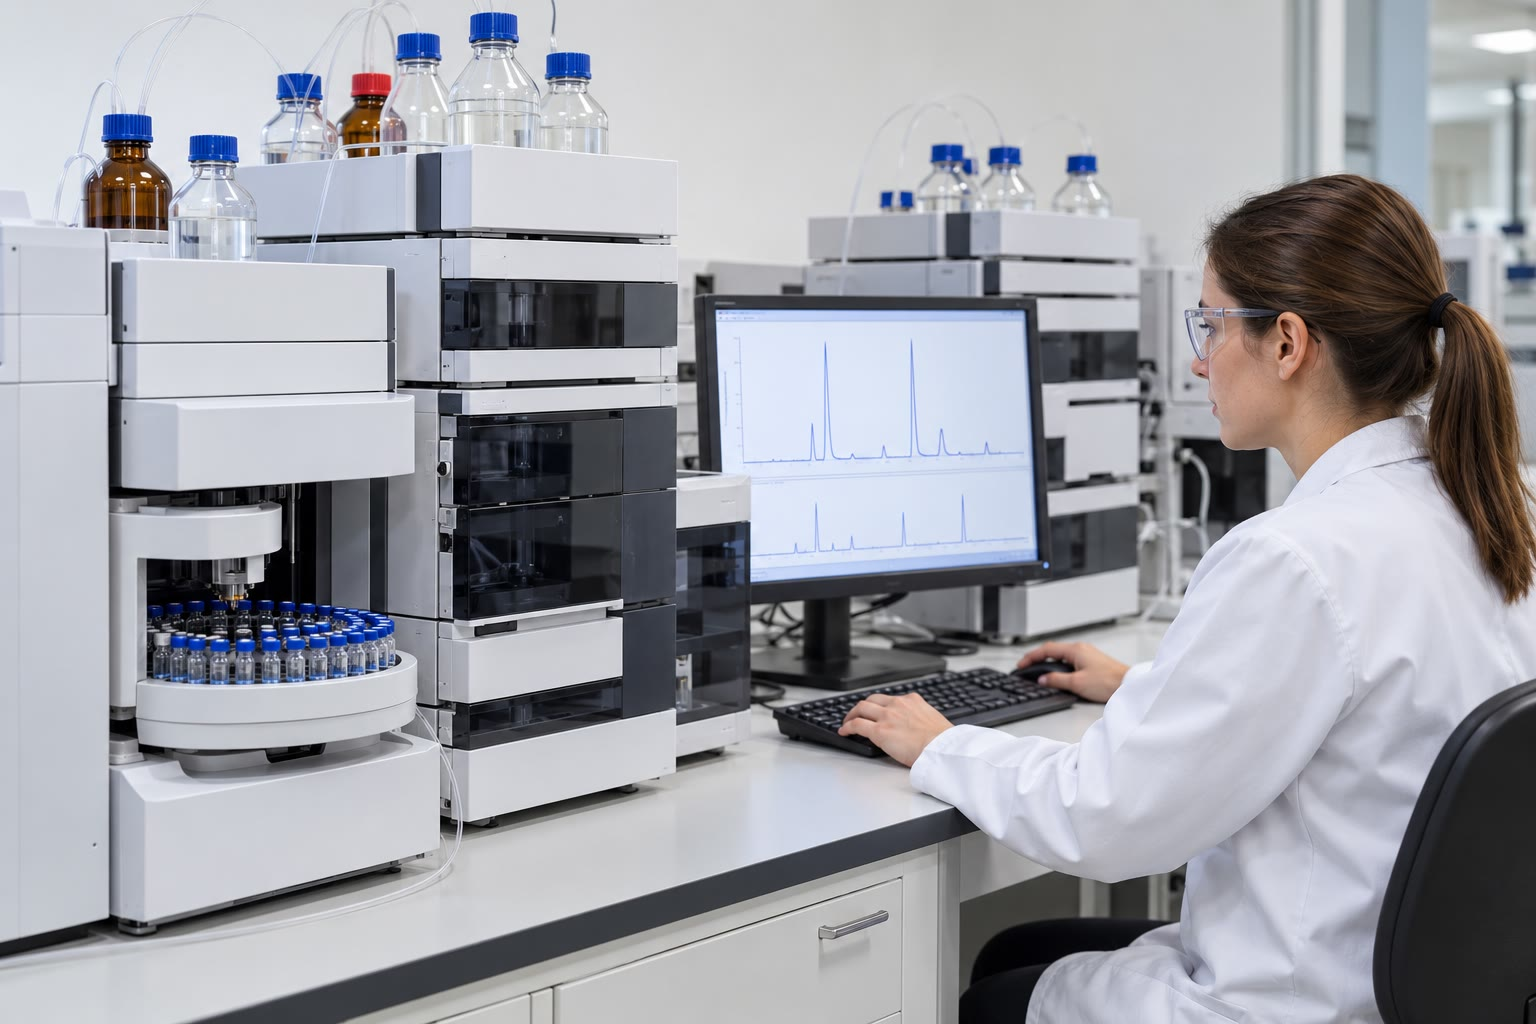
\includegraphics[width=0.58\linewidth]{images/book3/ai/b2-31-analytical-lab.jpg}

{\small مختبر تحليلي: أجهزة \omterm{def:b2:chromatography:principle}{كروماتوغرافيا} سائلة مع قوارير مذيباتها وصينية حاقن آلي
من القوارير الصغيرة؛ وتظهر الكروماتوغرامات على الشاشة (رسم توضيحي).}
\end{omfigure}

\begin{recall}
المجلد المدرسي: \omterm{def:b2:chromatography:principle}{الكروماتوغرافيا} الورقية \omterm{def:b2:chromatography:principle}{والكروماتوغرافيا} على طبقة رقيقة، والكروماتوغرام، والمُزيح. ومجلد السنة الأولى:
معامل التوزيع، والاستخلاص سائل--سائل، \omterm{def:b2:chromatography:retention}{ومعامل الاحتجاز} $R_f$ لصفيحة الطبقة الرقيقة.
و\cref{ch:b2:liquid-vapour-diagrams}: \omterm{def:b2:liquid-vapour-diagrams:fractional-distillation}{الطبق النظري} لعمود التقطير.
\end{recall}

\section{المبدأ}

\begin{definition}[الكروماتوغرافيا]\label{def:b2:chromatography:principle}
\emph{الكروماتوغرافيا}\index{كروماتوغرافيا} تفصل مكونات خليط بتوزيعها
بين \emph{طور ثابت}\index{طور ثابت}، مثبت في عمود أو على صفيحة، 
و\emph{طور متحرك}\index{طور متحرك}، غاز أو سائل يجري بمحاذاته. وحمل المكونات
عبر العمود وإخراجها منه بالطور المتحرك هو \emph{الإزاحة}\index{إزاحة}.
\end{definition}

لا يتحرك الجزيء إلا ما دام في \omterm{def:b2:chromatography:principle}{الطور المتحرك}؛ وحين يمسكه \omterm{def:b2:chromatography:principle}{الطور الثابت}
ينتظر. وهو ينتقل بين الطورين ملايين المرات في طريقه، فتتحدد سرعته المتوسطة
بكسر الزمن الذي يقضيه في كل منهما، أي بتوازن توزعه.

\begin{definition}[الاحتجاز]\label{def:b2:chromatography:retention}
\emph{زمن الاحتجاز}\index{زمن الاحتجاز} $t_R$ لمركب هو الزمن من الحقن حتى
قمة ذروته؛ و\emph{الزمن الميت}\index{زمن ميت} $t_M$ هو زمن الاحتجاز لمركب
غير محتجز، لا يدخل \omterm{def:b2:chromatography:principle}{الطور الثابت} أبدًا. و\emph{معامل الاحتجاز}\index{معامل الاحتجاز k@معامل الاحتجاز $k$}
$k$ لمركب على عمود هو
\begin{equation*}
k = \frac{t_R - t_M}{t_M}.
\end{equation*}
وهو ليس $R_f$ لصفيحة الطبقة الرقيقة، الذي يقيس مسافة مقطوعة، وإن كان كلاهما يصف
التوزع نفسه.
\end{definition}

\begin{proposition}[زمن الاحتجاز]\label{prop:b2:chromatography:retention-time}
إذا كانت كميتا مركب في الطورين الثابت والمتحرك لشريحة من العمود عند التوازن
$n_s$ و$n_m$، فإن المركب يتحرك بالسرعة $u/(1 + n_s/n_m)$، حيث $u$ سرعة \omterm{def:b2:chromatography:principle}{الطور المتحرك}،
و$t_R = t_M(1 + n_s/n_m)$.
\end{proposition}

\begin{proof}
يقضي جزيء معين الكسر $n_m/(n_s + n_m)$ من وقته في \omterm{def:b2:chromatography:principle}{الطور المتحرك}، حيث يتحرك بالسرعة
$u$، ويبقى ساكنًا في الباقي. فسرعته المتوسطة $u\,n_m/(n_s + n_m) = u/(1 + n_s/n_m)$. ويُقطع العمود ذو
الطول $L$ في $t_R = (L/u)(1 + n_s/n_m)$، و$L/u = t_M$.
\end{proof}

\begin{proposition}[الاحتجاز والتوزع]\label{prop:b2:chromatography:k-and-K}
\omterm{def:b2:chromatography:retention}{معامل الاحتجاز} هو نسبة الكميتين في الطورين، $k = n_s/n_m = KV_s/V_m$، حيث $K$
معامل التوزع (التركيز في \omterm{def:b2:chromatography:principle}{الطور الثابت} على التركيز في \omterm{def:b2:chromatography:principle}{الطور
المتحرك}) و$V_s$، $V_m$ حجما الطورين في العمود.
\end{proposition}

\begin{proof}
من \cref{prop:b2:chromatography:retention-time}، $(t_R - t_M)/t_M = n_s/n_m$. ومع $n_s = c_sV_s$،
$n_m = c_mV_m$ و$K = c_s/c_m$، $n_s/n_m = KV_s/V_m$.
\end{proof}

ينفصل مركبان إذا اختلف معاملا توزعهما؛ أما هندسة العمود ($V_s/V_m$)
فتضرب كل الاحتجازات بالعامل نفسه. وتغيير \omterm{def:b2:chromatography:principle}{الطور المتحرك}، الذي يغيّر $K$، هو الرافعة الرئيسية
للكيميائي على الاحتجاز.

\begin{omfigure}
\begin{tikzpicture}[x=1cm, y=1cm]
\foreach \x/\a/\b/\ha/\hb/\lab in {0/0.6/0.6/0.1/0.1/البداية, 2.4/1.5/2.6/0.16/0.22/لاحقًا, 4.8/2.4/4.4/0.2/0.3/النهاية}{
  \draw[black!60] (\x-0.35,0) rectangle (\x+0.35,-5);
  \fill[omThm!55] (\x-0.33,-\b+\hb) rectangle (\x+0.33,-\b-\hb);
  \fill[omDef!55, opacity=0.85] (\x-0.33,-\a+\ha) rectangle (\x+0.33,-\a-\ha);
  \node[font=\small] at (\x,-5.4) {\lab};
}
\draw[->, thick] (-1.0,-0.3) -- (-1.0,-4.6) node[midway, left, font=\small, align=right] {الطور\\المتحرك};
\node[font=\small, align=left, anchor=west] at (5.5,-2.4) {\shortstack{\foreignlanguage{arabic}{أكثر احتجازًا}\\\foreignlanguage{arabic}{(بطيء، ضيق)}}};
\node[font=\small, align=left, anchor=west] at (5.5,-4.4) {\shortstack{\foreignlanguage{arabic}{أقل احتجازًا}\\\foreignlanguage{arabic}{(سريع)}}};
\draw[densely dotted] (5.15,-2.4) -- (5.5,-2.4); \draw[densely dotted] (5.15,-4.4) -- (5.5,-4.4);
\end{tikzpicture}
\par\vspace{4pt}

{\small مركبان حُقنا معًا على هيئة نطاق رقيق واحد يتحركان نزولًا في عمود (ثلاث لقطات،
رسم تخطيطي). الأقل احتجازًا (ذو $k$ الأصغر) يسبق الآخر؛ ويتسع النطاقان كلاهما في أثناء سيرهما، والذي
قطع مسافة أطول أكثر من الآخر.}
\end{omfigure}

\section{عرض القمة وعدد الأطباق}

لا يبقى النطاق رقيقًا. فجزيئات المركب نفسه تسلك مسارات مختلفة بين الحبيبات،
وتنتشر على طول العمود وتتأخر في \omterm{def:b2:chromatography:principle}{الطور الثابت} بمقادير عشوائية. والقمة المسجلة عند
المخرج دالة غاوس تقريبًا انحرافها المعياري $\sigma_t$ (زمنًا)، وكلما كانت أضيق
من أجل $t_R$ معطاة، كان العمود أفضل.

\begin{definition}[عدد الأطباق]\label{def:b2:chromatography:plates}
\emph{عدد الأطباق}\index{عدد الأطباق} لعمود بالنسبة إلى مركب هو $N = (t_R/\sigma_t)^2$، حيث
$\sigma_t$ الانحراف المعياري لقمته زمنًا. و\emph{ارتفاع الطبق}\index{ارتفاع الطبق} هو
$H = L/N$، لعمود طوله $L$.
\end{definition}

تأتي التسميات من عمود التقطير في \cref{ch:b2:liquid-vapour-diagrams}: فالعمود الكروماتوغرافي
يسلك كما لو كان كومة من $N$ مرحلة توازن، ارتفاع كل منها $H$. والتشبيه طريقة
في العدّ، لا صورة للعمود.

\begin{proposition}[عدد الأطباق من قمة]\label{prop:b2:chromatography:plate-number}
مع $w$ العرض عند القاعدة بين المماسين عند نقطتي الانعطاف و$w_{1/2}$ العرض عند
منتصف الارتفاع،
\begin{equation*}
N = 16\left(\frac{t_R}{w}\right)^2 = 5.54\left(\frac{t_R}{w_{1/2}}\right)^2.
\end{equation*}
\end{proposition}

\begin{proof}
من أجل دالة غاوس انحرافها المعياري $\sigma$ وارتفاعها $h$، تقع نقطتا الانعطاف عند $\pm\sigma$،
حيث الارتفاع $h\mathrm e^{-1/2}$ والميل $\mp h\mathrm e^{-1/2}/\sigma$؛ والمماس هناك
يبلغ الصفر بعد $\sigma$ إضافية، عند $\pm2\sigma$: $w = 4\sigma$. ويُبلغ منتصف الارتفاع حيث
$\mathrm e^{-x^2/2\sigma^2} = 1/2$، $x = \sigma\sqrt{2\ln2}$: $w_{1/2} = 2\sqrt{2\ln2}\,\sigma \approx
2.355\,\sigma$. وبالتعويض $\sigma = w/4$ أو $\sigma = w_{1/2}/2.355$ في $N = (t_R/\sigma)^2$ نحصل على
$16$ و$2.355^2 = 5.545$، المكتوبة 5.54.
\end{proof}

\begin{proposition}[معادلة فان ديمتر]\label{prop:b2:chromatography:van-deemter}
يتعلق \omterm{def:b2:chromatography:plates}{ارتفاع الطبق} بالسرعة الخطية $u$ \omterm{def:b2:chromatography:principle}{للطور المتحرك} وفق
\begin{equation*}
H = A + \frac{B}{u} + Cu,
\end{equation*}
حيث يعبّر $A$ عن اختلاف المسارات عبر الحشوة، و$B/u$ عن الانتشار على طول العمود
(أسوأ حين تمكث الجزيئات أطول) و$Cu$ عن بطء التبادل مع \omterm{def:b2:chromatography:principle}{الطور الثابت} (أسوأ
حين يسرع \omterm{def:b2:chromatography:principle}{الطور المتحرك} بمحاذاته). ويكون $H$ أصغر ما يمكن عند $u_{\mathrm{opt}} = \sqrt{B/C}$، حيث $H_{\min} =
A + 2\sqrt{BC}$.
\end{proposition}

\admitted

شكل المعادلة مقبول هنا؛ أما قيمتها الصغرى فلا. فالمشتق $\mathrm dH/\mathrm du = -B/u^2 + C$ ينعدم
عند $u = \sqrt{B/C}$، وهناك $B/u = Cu = \sqrt{BC}$، إذن $H_{\min} = A + 2\sqrt{BC}$؛ والمشتق
الثاني $2B/u^3$ موجب، فهذه قيمة صغرى. والحبيبات الصغيرة تخفض $A$ و$C$: ولهذا
تستعمل \omterm{def:b2:chromatography:principle}{الكروماتوغرافيا} السائلة الحديثة جسيمات من بضعة ميكرومترات وضغوطًا مرتفعة لدفع \omterm{def:b2:chromatography:principle}{الطور
المتحرك} عبرها.

\begin{omfigure}
\begin{tikzpicture}
\begin{axis}[width=0.7\linewidth, height=5.2cm, xmin=0, xmax=8, ymin=0, ymax=70,
  xlabel={\foreignlanguage{arabic}{السرعة الخطية $u$ \babelsublr{(\unit{mm/s})}}}, ylabel={\foreignlanguage{arabic}{ارتفاع الطبق $H$ \babelsublr{(\unit{\micro m})}}},
  label style={font=\small}, tick label style={font=\scriptsize},
  legend style={font=\scriptsize, at={(1.03,1)}, anchor=north west}, legend cell align=left]
\addplot[omDef, very thick] table[x=u, y=H] {figdata/out/bachelor-2-chromatogram-b.dat};
\addplot[black!50, dashed] table[x=u, y=A] {figdata/out/bachelor-2-chromatogram-b.dat};
\addplot[omThm, dashed] table[x=u, y=B] {figdata/out/bachelor-2-chromatogram-b.dat};
\addplot[omMeth, dashed] table[x=u, y=C] {figdata/out/bachelor-2-chromatogram-b.dat};
\addplot[only marks, mark=*, mark size=1.6pt] coordinates {(2,30)};
\legend{$H$, $A$, $B/u$, $Cu$}
\end{axis}
\end{tikzpicture}

{\small منحنى فان ديمتر (وسائط تمرين: $A = \qty{10}{\micro m}$، $B = \qty{20}{\micro m.mm/s}$،
$C = \qty{5}{\micro m.s/mm}$). والقيمة الصغرى، $H = \qty{30}{\micro m}$ عند $u = \qty{2}{mm/s}$، تقع حيث
يتساوى حدّا الانتشار والتبادل.}
% figdata: bachelor-2/chromatogram.py part b
\end{omfigure}

\section{فصل مركبين}

\begin{definition}[الانتقائية والميز]\label{def:b2:chromatography:separation}
من أجل قمتين متجاورتين مع $k_2 > k_1$، يكون \emph{معامل الانتقائية}\index{معامل الانتقائية}
$\alpha = k_2/k_1$، و\emph{الميز}\index{ميز} هو
\begin{equation*}
R_s = \frac{2(t_{R2} - t_{R1})}{w_1 + w_2},
\end{equation*}
أي المسافة بين القمتين مقسومة على متوسط عرضيهما عند القاعدة.
\end{definition}

عند $R_s = 1$ تبقى القمتان متداخلتين على نحو مرئي؛ وعند $R_s = 1.5$ تعود الإشارة إلى خط الأساس بينهما
(فصل حتى خط الأساس)، وهو الهدف المعتاد في العمل الكمي.

\begin{omfigure}
\begin{tikzpicture}
\begin{axis}[width=0.36\linewidth, height=3.6cm, xmin=-8, xmax=8, ymin=0, ymax=1.15,
  xtick=\empty, ytick=\empty, axis x line=bottom, axis y line=none, title style={font=\small},
  title={$R_s = 0.75$}]
\addplot[omDef, thick] table[x=x, y=r075] {figdata/out/bachelor-2-chromatogram-a.dat};
\end{axis}
\end{tikzpicture}\hfill\begin{tikzpicture}
\begin{axis}[width=0.36\linewidth, height=3.6cm, xmin=-8, xmax=8, ymin=0, ymax=1.15,
  xtick=\empty, ytick=\empty, axis x line=bottom, axis y line=none, title style={font=\small},
  title={$R_s = 1.0$}]
\addplot[omDef, thick] table[x=x, y=r100] {figdata/out/bachelor-2-chromatogram-a.dat};
\end{axis}
\end{tikzpicture}\hfill\begin{tikzpicture}
\begin{axis}[width=0.36\linewidth, height=3.6cm, xmin=-8, xmax=8, ymin=0, ymax=1.15,
  xtick=\empty, ytick=\empty, axis x line=bottom, axis y line=none, title style={font=\small},
  title={$R_s = 1.5$}]
\addplot[omDef, thick] table[x=x, y=r150] {figdata/out/bachelor-2-chromatogram-a.dat};
\end{axis}
\end{tikzpicture}

{\small قمتان غاوسيتان متساويتا الحجم عند ثلاث قيم \omterm{def:b2:chromatography:separation}{للميز} (نموذج). عند 0.75 تندمجان في
قمة مزدوجة؛ وعند 1.0 يبقى الوادي عند ربع الارتفاع؛ وعند 1.5 تعود الإشارة إلى
خط الأساس.}
% figdata: bachelor-2/chromatogram.py part a
\end{omfigure}

\begin{theorem}[معادلة الميز]\label{thm:b2:chromatography:resolution}
من أجل قمتين متجاورتين لهما \omterm{def:b2:chromatography:plates}{عدد الأطباق} نفسه $N$،
\begin{equation*}
R_s = \frac{\sqrt N}{4}\,\frac{\alpha - 1}{\alpha}\,\frac{k_2}{1 + k_2}.
\end{equation*}
\end{theorem}

\begin{proof}
من أجل قمتين متقاربتين يكون عرضا القاعدة متساويين تقريبًا؛ فلنأخذهما مساويين لعرض القمة الثانية،
$w = 4\sigma_t = 4t_{R2}/\sqrt N$ (\cref{def:b2:chromatography:plates}). عندئذ $R_s = (t_{R2} -
t_{R1})/w = \sqrt N\,(t_{R2} - t_{R1})/(4t_{R2})$. ومع $t_R = t_M(1 + k)$
(\cref{prop:b2:chromatography:retention-time})، $t_{R2} - t_{R1} = t_M(k_2 - k_1)$ و$t_{R2} =
t_M(1 + k_2)$، إذن $R_s = (\sqrt N/4)(k_2 - k_1)/(1 + k_2)$. وأخيرًا $k_2 - k_1 = k_2(1 - 1/\alpha) =
k_2(\alpha - 1)/\alpha$.
\end{proof}

\begin{method}[تحسين الميز]\label{met:b2:chromatography:improve-resolution}
\begin{enumerate}
  \item الكفاءة: $R_s \propto \sqrt N$. ومضاعفة طول العمود تضاعف $N$ وزمن التحليل
        لكنها لا تضرب $R_s$ إلا في $\sqrt2 \approx 1.41$؛ والجسيمات الأصغر أو معدل التدفق الأمثل
        يرفعان $N$ عند طول ثابت.
  \item الانتقائية: العامل $(\alpha - 1)/\alpha$ هو الأشد حساسية. غيّر \omterm{def:b2:chromatography:principle}{الطور المتحرك}
        (المذيب، pH)، أو \omterm{def:b2:chromatography:principle}{الطور الثابت} أو، في \omterm{def:b2:chromatography:techniques}{كروماتوغرافيا الغاز}، درجة الحرارة.
  \item الاحتجاز: يرتفع $k_2/(1+k_2)$ بحدة حتى $k \approx 2$ ثم ببطء بعد ذلك، بينما يواصل الزمن
        نموه بمقدار $1 + k$؛ فاستهدف $k$ بين نحو 2 و10.
\end{enumerate}
\end{method}

\section{التقنيات}

\begin{definition}[التقنيات الكروماتوغرافية]\label{def:b2:chromatography:techniques}
في \emph{كروماتوغرافيا الغاز}\index{كروماتوغرافيا الغاز} (GC)، يكون \omterm{def:b2:chromatography:principle}{الطور المتحرك} غازًا (الهيليوم، أو الهيدروجين
أو النيتروجين) \omterm{def:b2:chromatography:principle}{والطور الثابت} غشاءً سائلًا يكسو داخل عمود شعري طويل، محفوظ
في فرن. وفي \emph{الكروماتوغرافيا السائلة العالية الأداء}\index{كروماتوغرافيا سائلة عالية الأداء}
(HPLC)، تدفع مضخة طورًا متحركًا سائلًا عبر عمود قصير محشو بجسيمات
صغيرة. وفي HPLC \emph{بالطور المعكوس}\index{طور معكوس}، يكون \omterm{def:b2:chromatography:principle}{الطور الثابت} غير قطبي
(سيليكا تحمل سلاسل ألكيلية طويلة) \omterm{def:b2:chromatography:principle}{والطور المتحرك} خليطًا قطبيًا من الماء مع الميثانول أو
الأسيتونتريل. وفي \emph{الإزاحة المتدرجة}\index{إزاحة متدرجة}، يُغيَّر تركيب \omterm{def:b2:chromatography:principle}{الطور المتحرك}
أثناء التشغيل، في \omterm{def:b2:chromatography:principle}{الكروماتوغرافيا} السائلة، \omterm{def:b2:chromatography:principle}{لإزاحة} المركبات الشديدة الاحتجاز أسرع.
\end{definition}

\begin{omfigure}
\begin{tikzpicture}[x=1cm, y=1cm, box/.style={draw=black!70, rounded corners=2pt, fill=white,
  font=\small, align=center, minimum height=0.8cm, inner sep=3pt}]
\node[box] (gas) at (0,0) {غاز\\حامل};
\node[box] (inj) at (2.2,0) {حاقن\\مسخَّن};
\draw[black!70, rounded corners=2pt, fill=omDef!8] (3.5,-1.1) rectangle (6.5,1.1);
\node[font=\small] at (5,0.85) {فرن};
\draw[omDef, thick] (5,-0.15) circle (0.55); \draw[omDef, thick] (5,-0.15) circle (0.42);
\node[box] (det) at (8.0,0) {كاشف};
\node[box] (data) at (10.2,0) {نظام\\البيانات};
\draw[->, thick] (gas) -- (inj);
\draw[->, thick] (inj.east) -- (4.45,0);
\draw[->, thick] (5.55,0) -- (det.west);
\draw[->, thick] (det) -- (data);
\node[font=\footnotesize, align=center] at (5,-1.45) {\shortstack{\foreignlanguage{arabic}{عمود شعري (ملفوف)}}};
\end{tikzpicture}

\medskip
\begin{tikzpicture}[x=1cm, y=1cm, box/.style={draw=black!70, rounded corners=2pt, fill=white,
  font=\small, align=center, minimum height=0.8cm, inner sep=3pt}]
\node[box] (sol) at (0,0) {خزانات\\المذيبات};
\node[box] (pump) at (2.4,0) {مضخة\\عالية الضغط};
\node[box] (inj) at (4.9,0) {حاقن};
\draw[black!70, fill=omThm!12] (6.2,-0.18) rectangle (8.2,0.18);
\node[font=\footnotesize] at (7.2,0.45) {عمود محشو};
\node[box] (uv) at (9.6,0) {خلية\\\babelsublr{UV}};
\node[box] (data) at (11.5,0) {بيانات};
\draw[->, thick] (sol) -- (pump); \draw[->, thick] (pump) -- (inj);
\draw[->, thick] (inj) -- (6.2,0); \draw[->, thick] (8.2,0) -- (uv); \draw[->, thick] (uv) -- (data);
\end{tikzpicture}
\par\vspace{4pt}

{\small مخططات كتلية. في الأعلى: جهاز \omterm{def:b2:chromatography:techniques}{كروماتوغرافيا الغاز}؛ تتبخر العينة في الحاقن، ويحملها
الغاز عبر عمود شعري طوله عشرات الأمتار ملفوف في فرن، ويُكشف عنها عند المخرج.
وفي الأسفل: جهاز \omterm{def:b2:chromatography:principle}{كروماتوغرافيا} سائلة؛ تخلط المضخة المذيبات (\omterm{def:b2:chromatography:techniques}{إزاحة متدرجة}) وتدفعها بضغط
مرتفع عبر عمود محشو قصير إلى خلية امتصاص في الأشعة فوق البنفسجية.}
\end{omfigure}

يتحدد الاختيار بينهما بالتطاير. إذ تحتاج GC إلى مركبات تتبخر دون أن تتفكك،
أي تقريبًا دون \qty{400}{\degreeCelsius}: المذيبات، والوقود، والعطور، والجزيئات العضوية الصغيرة. ورفع
درجة حرارة الفرن أثناء التشغيل (منحدر حراري) يزيح المركبات الأثقل أسرع، كما يفعل التدرج
في HPLC. أما HPLC فتعالج كل ما يذوب، بما في ذلك الأملاح والسكريات والأدوية والبروتينات. وفي
\omterm{def:b2:chromatography:techniques}{الطور المعكوس} تخرج المركبات الأشد قطبية أولًا والأقل قطبية أخيرًا؛ وإضافة مزيد من المذيب
العضوي إلى \omterm{def:b2:chromatography:principle}{الطور المتحرك} تخفض كل الاحتجازات. \omterm{def:b2:chromatography:principle}{والكروماتوغرافيا} العمودية التحضيرية، ونسختها الأسرع،
\omterm{def:b2:chromatography:principle}{الكروماتوغرافيا} الومضية، تطبقان المبدأ نفسه على نطاق واسع لتنقية غرامات من الناتج،
عادة على سيليكا قطبية بخلائط من الهكسان وإيثانوات الإيثيل.

\section{التحليل الكمي}

مساحة القمة متناسبة مع كمية المركب التي بلغت الكاشف، لكن
ثابت التناسب يتعلق بالمركب وبالكاشف. والحجوم المحقونة، التي هي من رتبة
الميكرولتر، ليست قابلة للتكرار تمامًا. \omterm{def:b2:chromatography:quantitative}{والمعيار الداخلي} يزيل الصعوبتين كلتيهما.

\begin{definition}[معامل الاستجابة والمعيار الداخلي]\label{def:b2:chromatography:quantitative}
\emph{المعيار الداخلي}\index{معيار داخلي} مركب، غائب عن العينة، يُضاف بكمية
معلومة إلى كل محلول يُحلَّل؛ ويجب أن يكون مفصولًا عن كل القمم الأخرى وأن يسلك سلوك
المادة المحللة. و\emph{معامل الاستجابة}\index{معامل الاستجابة} $F$ للمادة المحللة بالنسبة إلى المعيار
الداخلي يُعرَّف بالعلاقة
\begin{equation*}
\frac{A_X}{A_{IS}} = F\,\frac{c_X}{c_{IS}},
\end{equation*}
حيث $A$ مساحات القمم و$c$ التراكيز في المحلول المحقون.
\end{definition}

\begin{proposition}[التقدير الكمي بالمعيار الداخلي]\label{prop:b2:chromatography:internal-standard}
$F$ المقيس على محلول معايرة معلوم $c_X$ و$c_{IS}$ يعطي، من أجل عينة أُضيف إليها
\omterm{def:b2:chromatography:quantitative}{المعيار الداخلي} بالتركيز $c_{IS}$، $c_X = (A_X/A_{IS})\,c_{IS}/F$، أيًّا كان الحجم المحقون.
\end{proposition}

\begin{proof}
كل مساحة متناسبة مع الكمية المحقونة: $A_X = s_X c_X v$، $A_{IS} = s_{IS} c_{IS} v$، مع
حساسيتي الكاشف $s$ والحجم المحقون $v$. والنسبة $A_X/A_{IS} = (s_X/s_{IS})(c_X/c_{IS})$
لم تعد تحوي $v$، و$F = s_X/s_{IS}$ ثابت للطريقة، يُقاس مرة واحدة على
محلول المعايرة. وحلّها لإيجاد $c_X$ يعطي النتيجة.
\end{proof}

\begin{method}[التقدير الكمي بمعيار داخلي]\label{met:b2:chromatography:internal-standard}
\begin{enumerate}
  \item اختر معيارًا قريب البنية من المادة المحللة، غائبًا عن العينة، يخرج قربها
        لكن مفصولًا عنها ($R_s \ge 1.5$).
  \item احقن محلول معايرة معلوم $c_X$ و$c_{IS}$؛ واحسب $F$ من نسبة المساحتين.
  \item أضف المعيار إلى محلول العينة بالتركيز نفسه $c_{IS}$؛ واحقن؛ واقرأ $A_X/A_{IS}$.
  \item احسب $c_X = (A_X/A_{IS})\,c_{IS}/F$، ثم عُد عبر كل تخفيف إلى العينة
        الأصلية.
\end{enumerate}
\end{method}

المعايرة الخارجية (سلسلة من معايير المادة المحللة وحدها، ثم العينة، وكلها تُحقن بالطريقة
نفسها) أبسط لكنها تعتمد على بقاء الحجم المحقون والكاشف ثابتين بين التشغيلات.

\begin{history}[الكتابة بالألوان، 1906]
\begin{minipage}[t]{0.18\linewidth}
\vspace{0pt}
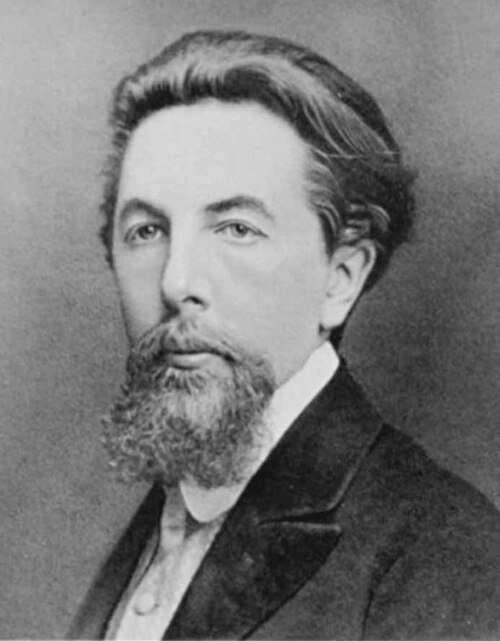
\includegraphics[width=\linewidth]{images/book3/tsvet.jpg}
\end{minipage}\hfill
\begin{minipage}[t]{0.78\linewidth}
\vspace{0pt}
صبّ عالم النبات ميخائيل تسفيت مستخلصًا من الأوراق الخضراء على أنبوب زجاجي مملوء بمسحوق
الطباشير وغسله بمذيب: فانفصلت الأصباغ في نطاقات ملوّنة، كلوروفيلات
خضراء وكاروتينات صفراء. وفي سنة 1906 سمّى الطريقة \omterm{def:b2:chromatography:principle}{الكروماتوغرافيا}، أي «الكتابة بالألوان».
وظلت مهملة إلى حد بعيد ربع قرن، حتى استُعيدت لدراسة المنتجات الطبيعية في
الثلاثينيات. (صورة شخصية: مؤلف مجهول، ملكية عامة؛ ويكيميديا كومنز.)
\end{minipage}
\end{history}

\begin{safety}{\ghs[5mm]{GHS02}\,\ghs[5mm]{GHS05}\,\ghs[5mm]{GHS06}\,\ghs[5mm]{GHS07}\,\ghs[5mm]{GHS08}\,\ghs[5mm]{GHS09}}
الأسيتونتريل والميثانول، المكوّنان العضويان المعتادان للأطوار المتحركة في HPLC، قابلان للاشتعال وسامّان؛
والهكسان، المستعمل في \omterm{def:b2:chromatography:principle}{الكروماتوغرافيا} العمودية، قابل للاشتعال وخطر على الصحة وسام للأحياء المائية.
وتُجمع نفايات المذيبات، ولا تُسكب أبدًا في المجرى.
% ledger: ghs:acetonitrile, ghs:methanol, ghs:hexane
\end{safety}

\section{تمارين}

\begin{exercise}[$\star$]\label{exo:b2:chromatography:1}
لمركب $t_R = \qty{5.0}{min}$ على عمود زمنه الميت \qty{1.0}{min}. احسب
معامل احتجازه وكسر الزمن الذي يقضيه في \omterm{def:b2:chromatography:principle}{الطور المتحرك}.
\end{exercise}

\begin{exercise}[$\star$]\label{exo:b2:chromatography:2}
قمة عند $t_R = \qty{6.0}{min}$ عرضها عند القاعدة \qty{0.30}{min}. احسب \omterm{def:b2:chromatography:plates}{عدد الأطباق}.
\end{exercise}

\begin{exercise}[$\star$]\label{exo:b2:chromatography:3}
يعطي عمود طوله \qty{250}{mm} القيمة $N = 10\,000$ لمركب. احسب \omterm{def:b2:chromatography:plates}{ارتفاع الطبق}.
\end{exercise}

\begin{exercise}[$\star$]\label{exo:b2:chromatography:4}
GC أم HPLC؟ الإيثانول في الدم؛ وبروتين؛ والكافيين في مشروب؛ والبنزين في وقود السيارات؛ والسكريات في عصير الفاكهة.
\end{exercise}

\begin{exercise}[$\star\star$]\label{exo:b2:chromatography:5}
قمتان: $t_{R1} = \qty{4.0}{min}$، $w_1 = \qty{0.40}{min}$؛ $t_{R2} = \qty{4.6}{min}$، $w_2 =
\qty{0.50}{min}$. احسب \omterm{def:b2:chromatography:separation}{الميز}. هل هما مفصولتان حتى خط الأساس؟
\end{exercise}

\begin{exercise}[$\star\star$]\label{exo:b2:chromatography:6}
كم طبقًا يلزم لفصل مركبين مع $\alpha = 1.10$ و$k_2 = 4.0$ عند
$R_s = 1.5$؟
\end{exercise}

\begin{exercise}[$\star\star$]\label{exo:b2:chromatography:7}
لعمود $A = \qty{5}{\micro m}$، $B = \qty{8}{\micro m.mm/s}$، $C = \qty{2}{\micro m.s/mm}$
(معطيات التمرين). أوجد السرعة المثلى وأصغر ارتفاع للطبق.
\end{exercise}

\begin{exercise}[$\star\star$]\label{exo:b2:chromatography:8}
تنبأ بترتيب خروج البنزين والفينول والتولوين في HPLC \omterm{def:b2:chromatography:techniques}{بالطور المعكوس} مع \omterm{def:b2:chromatography:principle}{طور متحرك}
ماء--ميثانول، وبما يحدث حين يُرفع كسر الميثانول.
\end{exercise}

\begin{exercise}[$\star\star$]\label{exo:b2:chromatography:9}
يعطي محلول معايرة لمادة محللة تركيزها \qty{20.0}{mg/L} مع \omterm{def:b2:chromatography:quantitative}{المعيار الداخلي} بتركيز \qty{10.0}{mg/L}
المساحتين 860 و400. وتعطي عينة أُضيف إليها المعيار بتركيز \qty{10.0}{mg/L} المساحتين 645 و410.
احسب \omterm{def:b2:chromatography:quantitative}{معامل الاستجابة} وتركيز المادة المحللة (معطيات التمرين).
\end{exercise}

\begin{exercise}[$\star\star\star$]\label{exo:b2:chromatography:10}
يعطي فصلٌ القيمة $R_s = 1.06$. أي طول للعمود، بالنسبة إلى الطول الحالي، يعطي $R_s = 1.5$، 
وما كلفة ذلك من الزمن؟ وما الروافع الأخرى المتاحة؟
\end{exercise}

\begin{exercise}[$\star\star\star$]\label{exo:b2:chromatography:11}
من أجل قمتين غاوسيتين متساويتي الارتفاع والعرض عرضهما عند القاعدة $w = 4\sigma$، احسب الإشارة
في منتصف المسافة بينهما، بالنسبة إلى ارتفاع القمة، عند $R_s = 1$ وعند $R_s = 1.5$ (أهمل مساهمة القمة
البعيدة عند كل قيمة عظمى).
\end{exercise}

\begin{exercise}[$\star\star\star$]\label{exo:b2:chromatography:12}
عند $N$ و$\alpha$ ثابتين، قارن عامل \omterm{def:b2:chromatography:separation}{الميز} $k_2/(1+k_2)$ وزمن التحليل النسبي
$1 + k_2$ من أجل $k_2 = 2$، 5 و10. أي مجال من $k$ تختار؟
\end{exercise}

\section{مسألة: الكافيين في مشروب طاقة}

\begin{problem}[{مسألة نهاية الأسبوع --- ترتيب الإزاحة في الطور المعكوس، وأداء العمود من
كروماتوغرام، وتحسين الفصل، والتقدير الكمي بمعيار داخلي}]
\label{pb:b2:chromatography:1}
معطيات تمرين (مختلقة، ليست طريقة حقيقية). يُخفف مشروب طاقة عشر مرات (\qty{5.00}{mL} إلى
\qty{50.0}{mL}) ويُضاف الثيوفيلين معيارًا داخليًا بتركيز \qty{40.0}{mg/L} في المحلول
المخفف. العمود: \qty{150}{mm}، \omterm{def:b2:chromatography:techniques}{طور معكوس}؛ \omterm{def:b2:chromatography:principle}{والطور المتحرك} ماء--ميثانول؛ والكشف بالأشعة فوق البنفسجية.
وتخرج مكونات المصفوفة غير المحتجزة (السكريات والأملاح) عند $t_M = \qty{1.0}{min}$؛ والثيوفيلين عند
\qty{3.0}{min} (عرض القاعدة \qty{0.18}{min})؛ والكافيين عند \qty{3.4}{min} (عرض القاعدة \qty{0.20}{min}).
المعايرة: الكافيين \qty{50.0}{mg/L} والثيوفيلين \qty{40.0}{mg/L} يعطيان المساحتين 1500 و1000.
العينة: المساحتان 970 (الكافيين) و1010 (الثيوفيلين). وتحوي العلبة \qty{250}{mL}.
% ledger: ghs:caffeine, ghs:methanol

\begin{center}
\begin{tikzpicture}
\begin{axis}[width=0.75\linewidth, height=4.4cm, xmin=0, xmax=5, ymin=0, ymax=1,
  xlabel={\foreignlanguage{arabic}{الزمن \babelsublr{(min)}}}, ylabel={\shortstack{\foreignlanguage{arabic}{الامتصاصية (بوحدات اعتباطية)}}}, label style={font=\small},
  tick label style={font=\scriptsize}, ytick=\empty]
\addplot[omDef, thick] table[x=t, y=s] {figdata/out/bachelor-2-chromatogram-c.dat};
\node[font=\scriptsize] at (axis cs:1.0,0.42) {المصفوفة};
\node[font=\scriptsize] at (axis cs:2.62,0.86) {الثيوفيلين};
\node[font=\scriptsize] at (axis cs:3.85,0.84) {الكافيين};
\end{axis}
\end{tikzpicture}
\end{center}
% figdata: bachelor-2/chromatogram.py part c

\medskip
\noindent\textbf{الجزء الأول --- \omterm{def:b2:chromatography:techniques}{الطور المعكوس}.}
\begin{enumerate}
  \item صف الطورين الثابت والمتحرك لعمود \omterm{def:b2:chromatography:techniques}{الطور المعكوس}.
  \item لماذا تخرج السكريات عند \omterm{def:b2:chromatography:retention}{الزمن الميت}؟
  \item الكافيين هو 1،3،7-ثلاثي ميثيل الزانثين، والثيوفيلين 1،3-ثنائي ميثيل الزانثين. فسّر ترتيب
        خروجهما.
  \item لماذا يكون الثيوفيلين معيارًا داخليًا جيدًا هنا؟
  \item ماذا يحدث لزمني الاحتجاز كليهما لو رُفع كسر الميثانول؟
  \item ماذا يقيس \omterm{def:b2:chromatography:retention}{الزمن الميت}؟
\end{enumerate}

\medskip
\noindent\textbf{الجزء الثاني --- أداء العمود.}
\begin{enumerate}[resume]
  \item احسب معاملي الاحتجاز للثيوفيلين والكافيين.
  \item احسب \omterm{def:b2:chromatography:separation}{معامل الانتقائية}.
  \item احسب \omterm{def:b2:chromatography:plates}{عدد الأطباق} للكافيين وللثيوفيلين.
  \item احسب \omterm{def:b2:chromatography:plates}{ارتفاع الطبق} للكافيين.
  \item احسب \omterm{def:b2:chromatography:separation}{الميز} بين القمتين.
  \item تحقق منه بمعادلة \omterm{def:b2:chromatography:separation}{الميز}.
  \item هل القمتان مفصولتان حتى خط الأساس؟
\end{enumerate}

\medskip
\noindent\textbf{الجزء الثالث --- أسرع أم أفضل.}
\begin{enumerate}[resume]
  \item لتوفير الوقت، يُقصَّر العمود إلى \qty{75}{mm} (الحشوة والتدفق نفساهما). ماذا يصير
        \omterm{def:b2:chromatography:separation}{الميز}؟
  \item وزمن التحليل؟
  \item ماذا كان سيعطي عمود طوله \qty{300}{mm} بدلًا من ذلك، وبأي كلفة؟
  \item أي رافعة تؤثر في $\alpha$؟
  \item هل تفيد زيادة $k$ كثيرًا هنا؟
\end{enumerate}

\medskip
\noindent\textbf{الجزء الرابع --- التقدير الكمي.}
\begin{enumerate}[resume]
  \item احسب \omterm{def:b2:chromatography:quantitative}{معامل الاستجابة} للكافيين بالنسبة إلى الثيوفيلين.
  \item لماذا لا يهم الحجم المحقون؟
  \item احسب تركيز الكافيين في المحلول المخفف.
  \item احسب تركيز الكافيين في المشروب.
  \item ما الخلل الذي يحدث لو خرج مركب من المصفوفة مع الثيوفيلين في الوقت نفسه؟
  \item ماذا كانت ستتطلب المعايرة الخارجية بدلًا من ذلك؟
  \item اذكر كتلة الكافيين في علبة سعتها \qty{250}{mL}.
\end{enumerate}
\end{problem}
